\newcommand{\bmhExpertChapter}{EXPERTEN-\\REGELN}
\newcommand{\bmhExpertHeadline}{Experten-Regeln}
\newcommand{\bmhExpertToc}{Experten-Regeln}
\newcommand{\bmhExpert}{%

	\dropping{D}ieses Kapitel enthält die Experten-Regeln von \bmh. Ihr könnt jederzeit von den Basis-Regeln umsteigen. Der folgende Text setzt aber nicht voraus, dass ihr diese gelesen habt, sondern wiederholt alle nötigen Regeln.

	\bmhSection{Spielplan}
		Eine \keyword{Battlemap} ist ein roll- oder faltbarer Spielplan, der mit trocken abwischbaren Stiften beschriftet werden kann. Auf diesem Plan ist ein quadratisches Raster aus \keyword[Feld]{Feldern} vorgedruckt.

		Die vier Linien, die jedes Feld umschließen, werden \keyword[Kante]{Kanten} genannt. Die Punkte, an denen vier Kanten zusammenlaufen, heißen \keyword{Ecken}. Kanten und Ecken sind imaginäre Hilfsmittel und nehmen keinen eigenen Platz am Spielfeld ein: Jeder Punkt einer Kante gehört zu beiden Feldern. Ebenso gehört jede Ecke zu allen vier dort zusammenstoßenden Feldern.

		Die acht umgebenden Felder, mit denen ein Feld eine Kante oder Ecke teilt, sind an dieses \keyword{angrenzend}. Jene vier davon, mit denen es nur eine Ecke teilt, werden \keyword[*]{diagonal angrenzend} bezeichnet.

		\example{\bmh\ kann optional auch auf Spielplänen mit wabenförmigen Hex-Feldern gespielt werden. Jedes Feld hat dann nur sechs statt acht angrenzende Felder. Alle Regeln behalten ihre Gültigkeit, auch wenn sämtliche Beispiele und Missionen in diesem Band von Quadraten ausgehen. }

	\bmhSection{Rollen \& Missionen}
		\bmh~ist ein Spiel für 3--5 Mitspieler. Einer übernimmt die Rolle des \keyword[Spielleiter]{Spielleiters}\index{SL} (SL), die anderen werden als \keyword{Spieler} bezeichnet.

		Der SL wählt zu Spielbeginn eine \keyword{Mission} (ab \refPage{lMissions}), studiert deren Karte und zeichnet den hervorgehobenen \keyword{Eingangsbereich} auf die Battlemap. Die Spieler wählen inzwischen die Helden, die sie durch die Mission führen wollen (\refPage{lHeroes}). Ist das deren erste Mission, überträgten die Spieler die Spielwerte auf neue Heldenbögen (\refPage{lSheets}), ansonsten bringen die Helden ihre Werte, Ausrüstung und Erfahrung von vorangegangenen Missionen mit.

		Der SL bittet die Spieler, ihre Helden auf die im Missionstext angegebenen Startfelder zu stellen. Zu guter Letzt stellt der SL alle anderen Kreaturen auf den Spielplan, die sich ebenfalls im Eingangsbereich befinden, und liest den Prolog vor.

		Während der Mission ziehen die Spieler nur ihre Helden, während der SL alle anderen Kreaturen übernimmt.

	\bmhSection{Kreaturen}
		Jede Figur, die einzeln am Spielplan bewegt werden kann, wird als \keyword[Kreatur]{Kreatur} bezeichnet. Meistens sind das Individuen, aber manchmal repräsentiert eine Figur mehrere, kleinere Wesen. Jedes Feld kann nur von einer Kreatur belegt sein. Kreaturen füllen stets die gesamte, rechteckige \keyword{Grundfläche} ihrer Felder aus, auch wenn die benutze Spielfigur kleiner oder abgerundet sein sollte.

		\example{Der Krieger, der Magier, ein Skelett, ein Riese oder ein Käferschwarm sind Beispiele für Kreaturen.}

		\noindent
		Die \keyword[Held]{Helden} der Spieler sind auch Kreaturen, wenn auch ganz besondere. Alle Regeln, die für Kreaturen gelten, gelten auch für Helden. Nur wenn explizit von \say{Helden} gesprochen wird, betrifft das nur diese.

		\example{Es kann vorkommen, dass ein Spieler mehrere Kreaturen steuert, oder eine Kreatur den Spieler wechselt, etwa Gefolgsleute oder bezauberte Monster.}

		\noindent
		Alle Kreaturen, die Spieler steuern, gelten als mit einander \keyword{befreundet} -- egal wie lange sie sich bereits kennen. Ebenso sind alle Kreaturen, die der SL steuert, untereinander befreundet. Kreaturen, die nicht miteinander befreundet sind, sind \keyword{befeindet}.

		\example{Von zwei Spielern gesteuerte Krieger und Magier sind mit einander \say{befreundete Kreaturen}. Vom SL gesteuerte Skelette und Riesenratten sind auch mit einander \say{befreundete Kreaturen}. Der Magier und die Riesenratten sind \say{befeindet}.}

	\bmhSection{Attribute \& Proben}
		Die Spielwerte der Kreaturen werden \keyword[Attribut]{Attribute} genannt. Deren gibt es: \keyword{Stärke}\index{ST} (ST), \keyword{Abwehr}\index{AB} (AB), \keyword{Geschick}\index{GE} (GE), \keyword{Reflexe}\index{RE} (RE), \keyword{Intelligenz}\index{IN} (IN) und \keyword{Willenskraft}\index{WI} (WI).

		Ist eine Kreatur aufgefordert, ein Attribut auf die \keyword{Probe} zu stellen, würfelt ihr Spieler entsprechend viele Würfel. Es werden jene gezählt, die gerade Nummern aufweisen. So viele \keyword[Erfolg]{Erfolge} hat die Probe.

		\example{Hat eine Kreatur Stärke~3 und ihr Spieler würfelt 4, 1 und 6. Die 4 und 6 zählen als zwei Erfolge.}

		\noindent
		Sind Proben \keyword{erleichtert}, \zB~\say{GE+2}, oder \keyword{erschwert}, \zB~\say{IN-1}, werden entsprechend mehr oder weniger Würfel benutzt. Sollten nach Abzügen keine Würfel übrig bleiben, sind das automatisch 0 Erfolge.

	\backgroundFooterFig[6.6cm]{%
		\begin{multicols}{2}\raggedbottom
			\fftext\color{white}\bmhExpertBoxLOS%
		\end{multicols}
	}

	\bmhSection{Stufen \& Limits}
		Kreaturen und Missionen haben jeweils eine \keyword{Stufe}, die ihre Kompetenz bzw. Gefährlichkeit ausdrückt.

		Da nicht immer alle Helden die selbe Stufe haben, muss vor dem Spiel die passende Missionsstufe bestimmt werden: Dazu wird der gerundete Durchschnitt aller, an der Mission teilnehmenden Helden berechnet. Der SL muss eine Mission wählen, deren Stufe zur Gruppenstufe passt.

		\example{Für Heldengruppe der Stufen 2, 2, 2 und 3 sollte der SL eine Mission der Stufe \say{2} wählen, für eine Gruppe der Stufen 2, 3, 3 und 3 eine Mission der Stufe \say{3}.}

		\noindent
		Während der Mission gilt für alle Kreaturen ein \keyword{Bonus-Limit}: Keine Probe darf um mehr Würfel erleichtert werden, als die Missionsstufe beträgt. Überzählige Würfel verfallen einfach. Alle anderen stufenabhängigen Eigenschaften behalten Kreaturen jedoch und dürfen sie einsetzen, etwa besondere Fähigkeiten.

		\example{Aus Sicht der Helden bedeutet das, dass sich Veteranen aus Rücksicht gegenüber Neulingen etwas zurückhalten und sich Neulinge dafür besonders anstrengen, mit den Veteranen Schritt zu halten.}

	\bmhSection{Runden \& Züge}
		Das Spiel wird in \keyword[Runden]{Runden} abgehalten. Die Mitspieler kommen im Uhrzeigersinn, beginnend links vom SL, an die Reihe und führen für jede ihrer Kreaturen einen Zug aus. Der SL zieht als letzter, danach endet die Runde. Ein Mitspieler muss den Zug einer Kreatur abschließen, eher mit einer weiteren Kreatur gezogen wird. Ein Mitspieler muss mit allen seinen Kreaturen ziehen -- oder auf deren Zug verzichten -- ehe der nächste an die Reihe kommt.

		Der \keyword[Zug]{Zug} einer Kreatur besteht aus einer Folge von Aktionen, die dessen Spieler bestimmt und durchführt. Die Kreatur erhält dazu so viele \keyword{Aktionspunkte}, wie ihr AP-Wert beträgt.

		Jede \keyword{Aktion} kostet AP. Eine Kreatur muss nicht alle Aktionen zu Beginn des Zuges ansagen, sondern kann den Ausgang einer abwarten, ehe er weitere setzt. Kreaturen können maximal einen unverbrauchten AP \keyword{ansparen} und in die nächste Runde mitnehmen. Alle anderen AP verfallen am Ende eines Zuges. APs können nicht an andere Kreaturen übertragen werden.

	\bmhSection{Aktionen}
		Kreaturen können folgende Aktionen zu den angegebenen Kosten durchführen:

		\medskip
		\bmhTable{X c}{
			\thead{Aktion} & \thead{AP} \\
		}{
			Angreifen           & 2 \\
			Benutzen            & 1 \\
			Bewegen             & 1 \\
			Fähigkeit einsetzen & 3 \\
			Falle entschärfen   & 2 \\
			Rückzug             & 1 \\
			Suchen              & 2 \\
		}
		\medskip

		\bmhSubsection{Angreifen -- 2AP}
			Kreaturen können nur Gegner angreifen, zu denen sie freie oder eingeschränkte Sicht haben (siehe Kasten). Außerdem muss der Gegner in der Reichweite ihrer Waffe stehen: Bestimme die \keyword{Distanz}, indem du die Felder zählst, die du minimal benötigst, um dieses auf direkter Linie horizontal, vertikal oder diagonal zu erreichen. Ignoriere dabei Hindernisse, Wände oder andere Kreaturen. Das Startfeld zählst du nicht mit, das Zielfeld schon.

			Jede Waffe hat eine \say{vs.}-Angabe. Diese bestimmt, mit welchen Attributen angegriffen und verteidigt wird.

			\example{Eine \say{ST vs. AB}-Waffe führst du mit deiner Stärke, dein Gegner verteidigt mit seiner Abwehr.}

			\noindent
			Hast eine Kreatur nur eingeschränkte Sicht auf ihren Gegner, muss sie mit einem Würfel weniger angreifen. Egal ob Schwert oder Zauberstab, alle Waffen funktionieren nach diesem Prinzip.

			Würfelt ein Mitspieler mehr Erfolge als der Gegner, hat er getroffen. Für jeden überzähligen Erfolg verliert der Gegner einen Lebenspunkt.

		\bmhSubsection{Benutzen -- 1AP}
			Mit dieser Aktion kann \emph{eine} Waffe, \emph{eine} Rüstung oder \emph{einen} Schild bereit gemacht, gewechselt oder weg gesteckt werden. Außerdem erlaubt sie, Gegenstände aus dem Inventar zu benutzen, etwa einen Trank zu trinken. Zu guter Letzt kannst mit dieser Aktion probiert werden, mit Gegenständen am Spielplan zu interagieren, etwa Schalter betätigen oder Gegenstände verschieben. Ob etwas bzw. was dann passiert, steht im Missionstext.

		\backgroundFooterFig[8.4cm]{%
			\begin{multicols}{2}\raggedbottom
				\fftext\color{white}\bmhExpertBoxExpose%
			\end{multicols}
		}

		\bmhSubsection{Bewegen -- 1AP}
			Pro Bewegungsaktion darf eine Kreatur Felder bis zu ihrem BEW-Wert weit gehen. Kreaturen bewegen sich dabei von Feld zu Feld und dürfen nicht durch geschlossene Türen oder Mauern gehen. Eine Kreatur darf ihre Bewegung nicht auf einem Feld beenden, auf dem bereits eine andere Kreatur steht. Ungenutzte BEW verfallen am Ende der Aktion.

			Sich ein Feld horizontal oder vertikal zu bewegen kostet 1 BEW. Sich diagonal zu bewegen kostet ebenfalls 1 BEW, ist aber nur dann erlaubt, wenn das Zielfeld über das horizontal oder vertikal dazwischen liegende Feld erreichbar wäre.

			Felder, die am Spielplan mit einem kleinen \say{x} markiert sind, gelten als \keyword{schwieriges Gelände}. Sie zu betreten kostet 1 BEW zusätzlich. Ein Feld, in dem eine andere Kreatur steht, gilt ebenso als schwieriges Gelände. Es zu passieren erfordert ihre Zustimmung.

			Kreaturen können 1 BEW ausgeben, um [liegend] zu werden oder 2 BEW ausgeben, um nicht mehr [liegend] zu sein. Kreaturen, die [liegend] sind, müssen beim Bewegen 1 BEW zusätzlich pro Feld bezahlen. Dafür erhalten sie u.U. Deckung (siehe Kasten \say{Sicht}).

			Eine Kreatur kann während deiner Bewegung 1 BEW ausgeben, um \keyword[Tür]{Türen zu öffnen oder zu schließen}, die sich auf einer Kante ihres Feldes befinden.

			Gegenstände aus dem eigenen oder einem angrenzenden Feld \keyword{aufheben oder ablegen} kostet 1 BEW pro Gegenstand.

			Zu versuchen, ein Feld nach oben zu klettern, kostet 2 BEW und erfordert eine ST\TN1 Probe. Misslingt die Probe, wird die Bewegung beendet, alle BEW verfallen und die Kreatur fällt. Sie verliert 1 LP pro Feld, dass sie fällt.

			Kann ein Held während deines Zuges \keyword[*]{neue Bereiche einsehen}, wird der SL die Karte vervollständigen (siehe Kasten \say{Aufdecken}).

		\bmhSubsection{Fähigkeit einsetzen -- 3AP}
			Die besonderen Fähigkeiten einer Kreatur einzusetzen ist zeitaufwändig und kostet 3AP. Kreaturen können diese Aktion nur ein mal pro Stufe in jeder Mission wählen. Die Effekte und Auswirkungen sind unter \say{Fähigkeiten} (\refPage{lPowers}) gelistet.

		\bmhSubsection{Falle entschärfen -- 2AP}
			Die Kreatur kann versuchen, eine Falle in einem angrenzenden Feld zu entschärfen. Sie legt dazu eine Probe ab, die in der Beschreibung der Falle angegeben ist. Gelingt sie, ist die Falle entschärft und wird von der Karte entfernt. Wird bei der Probe kein einziger Erfolg gewürfelt, löst die Falle aus.

		\bmhSubsection{Rückzug -- 1AP}
			Setzt ein Held auf einem der Startfelder die Aktion \keyword{Rückzug}, verlässt der en Spielplan und damit die Mission. Der Held ist dann in Sicherheit und streicht alle Zustände. Er nicht wieder in die Mission zurückkehren.

			Haben alle Helden die Mission verlassen, aber das Missionsziel ist noch nicht erfüllt, erhalten die Helden keine Belohnung.

		\bmhSubsection{Stoßen \& Bugsieren -- 1AP}
			Mit dieser Aktion können Kreaturen versuchen, nicht am Zug befindliche Kreaturen zu bewegen. Voraussetzung dafür ist, dass sich die zu bewegende Kreatur in einem benachbartem Feld in freier Sicht befindet.

			Der Angreifer hat die Wahl, ob er ST oder GE auf die Probe stellt, der Gegner darf zwischen AB oder GE wählen. Für jeden nicht abgewehrten Erfolg erhält der Angreifer 1 BEW. Diese darf dieser ausgeben, um den Gegner zu den regulären Regeln zu bewegen oder selbst in ein dadurch frei werdendes Feld nachzurücken. Angreifer und Gegner können auch die Plätze tauschen, wenn genügend BEW für beide Bewegungen gleichzeitig vorhanden sind.

		\bmhSubsection{Suchen -- 2AP}
			Sind keine Monster auf dem Spielplan, kann ein Held die Gelegenheit nutzen, um nach Verborgenem zu suchen. Dazu legt ihr Spieler den Suchradius fest: ein, zwei oder drei Felder. Durchsucht wird das Feld, auf dem die Kreatur steht, und alle Felder, die bis zu dieser Distanz in freier Sicht sind. Ob die Suche gelingt, entscheidet eine IN-Probe:

			\bmhTable{X c}{
				\thead{Suchradius} & \thead{nötige Erfolge} \\
			}{
				1 Feld    & 1 \\
				2 Felder  & 2 \\
				3 Felder  & 3 \\
			}

			\noindent
			Werden die nötigen Erfolge erzielt, nennt der SL alle Geheimnisse auf den durchsuchten Feldern. Gefundene Gegenstände müssen aber erst mit einer Bewegung aufgehoben werden.

			Gelingt die IN-Probe nicht, hast wurde nicht nur nichts gefunden, sondern \keyword[streunende Kreatur]{streunende Kreaturen}\index{Kreatur!streunend} aufgescheucht. Und zwar so viele, wie an Erfolgen fehlen. Durchsucht ein Held einen Radius von 3 Feldern und hat dabei nur einen Erfolg, werden zwei Kreaturen auf ihn aufmerksam! Im Missionstext ist angegeben, welche Kreaturen auftauchen. Der SL stellt sie auf angrenzende Felder (oder möglichst nahe, sollten alle Felder belegt sein).

	\bmhSection{Licht \& Schatten}
		Je nach verfügbarem Licht werden drei Grade an Helligkeit unterschieden:

		\keyword{Hell:} Es ist genügend Licht vorhanden, sodass alle Kreaturen ohne Einschränkungen ihre Aktionen durchführen können.

		\keyword{Düster:} Räume und deren Inhalt sind gerade noch auszumachen und werden vom SL normal eingezeichnet. Kreaturen in düsteren Feldern sind [getarnt] und [gehemmt].

		\keyword{Dunkel:} Es ist Nichts zu sehen. Der SL zeichnet nur Felder ein, die von Helden betreten und damit ertastet wurden. Kreaturen in dunklen Feldern sind [unsichtbar] und [hilflos].

		Jeder Raum bzw. jedes Areal auf dem Spielplan weist eine Grundhelligkeit auf. Ist in der Missionsbeschreibung nichts Gegenteiliges angegeben, so ist sie \say{Dunkel}.

		Kreaturen mit \keyword{Dunkelsicht} dürfen dunkle Felder wie düstere behandeln. Kreaturen mit \keyword{Düstersicht} dürfen düstere Felder wie helle behandeln.

		\bmhSubsection{Lichtquellen}
			Besitzt eine Kreatur eine transportable Lichtquelle, etwa eine Fackel oder Laterne, so erhöht sich die Helligkeit aller Felder in deren Reichweite um einen Grad, zu denen die Kreatur zumindest eingeschränkte Sicht hat. Erleuchten mindestens zwei Lichtquellen ein Feld, ist es \say{hell}.

			Fackeln und Lampen können auf dem Boden abgelegt werden, ohne dass sie erlöschen. Entzündete Fackeln oder Lampen halten bis zum Ende der Mission, müssen dann aber nachgekauft bzw. nachgefüllt werden.

	\bmhSection{Gegenangriffe}
		Kreaturen mit einer ST-Waffen bedrohen automatisch alle anderen Kreaturen in deren Reichweite, zu denen sie zumindest eingeschränkte Sicht haben. Löst eine bedrohte Kreatur eine der folgenden Ereignisse aus, erhält jede bedrohende Kreatur die Möglichkeit zum \keyword{Gegenangriff}:

		\bmhTable{X}{
			\thead{Ereignis im bedrohten Feld} \\
		}{
			Eine Kreatur gibt BEW aus. \\
			Eine Kreatur setzt die Aktion \say{Benutzen}. \\
			Eine Kreatur setzt die Aktion \say{Falle entschärfen}. \\
			Eine Kreatur setzt die Aktion \say{Fähigkeit einsetzen}. \\
		}

		\noindent
		Ein Gegenangriff kostet 1 AP und setzt daher voraus, dass die Kreatur einen Aktionspunkt angespart hat. Der Angriff findet statt, bevor die auslösende Kreatur ihre Aktion durchführt oder das Feld verlassen kann. Erst nachdem der Angriff komplett abgehandelt ist, darf die am Zug befindliche Kreatur fortfahren, sollte sie noch dazu in der Lage sein.

	\bmhSection{Zustände}
		Kreaturen können im Spiel temporäre Vor- und Nachteile erlangen. Diese werden \keyword{Zustände} genannt und sind im Text mit Klammern versehen, z.B. \tag{blind}. Eine Kreatur kann einen Zustand nicht mehrfach besitzen. Vor- oder Nachteile unterschiedlicher Zustände zählen gleichzeitig, aber es werden erst positive, danach die negativen verrechnet.

		\example{
			Eine Kreatur kann nicht zwei Mal \tag{schwach} sein, aber \tag{stark} und \tag{schwach}. Verliert diese Kreatur den Zustand \tag{schwach}, so ist sie nur noch \tag{stark}. Hat eine \tag{stark}e Kreatur noch eine weiteren Zustand, die ihr einen Stärke-Bonus gibt, addieren sich diese.
		}

		\bmhTable{l X}{
			\thead{Zustand} & \thead{Auswirkung}\\
		}{
			\tag{agil}         & GE+1, RE+1 \\
			\tag{blind}        & AB-1, RE-1, WI-1, keine Angriffe, kein Aufdecken \\
			\tag{gefangen}     & darf keine BEW ausgeben \\
			\tag{gehemmt}      & ST-1, GE-1, IN-1 \\
			\tag{getarnt}      & bestenfalls eingeschränkte Sicht \\
			\tag{hilflos}      & alle Proben haben 0 Erfolge \\
			\tag{konzentriert} & IN+1 und WI+1 \\
			\tag{langsam}      & BEW-2 \\
			\tag{liegend}      & keine Angriffe möglich \\
			\tag{schnell}      & BEW+2 \\
			\tag{schwach}      & ST-1, AB-1 \\
			\tag{stark}        & ST+1, AB+1 \\
			\tag{träge}        & GE-1, RE-1 \\
			\tag{unsichtbar}   & kann nicht angegriffen werden, kann Feinde passieren \\
			\tag{verflucht}    & verliert einmalig 1 LP am Ende des nächsten Zuges \\
			\tag{vergiftet}    & verliert 1 LP am Ende jedes Zuges \\
			\tag{verwirrt}     & IN-1, WI-1 \\
		}

	\bmhSection{Tote Kreaturen}
		Sinken die LP einer Kreatur auf 0, ist sie tot. Die Figur wird vom Spielplan genommen, die ehemalige Grundfläche der Kreatur ist nun schwieriges Gelände. Die Ausrüstung der Kreatur liegt nun ebenfalls auf dem Feld und kann von anderen Kreaturen aufgehoben werden.

	\bmhSection{Riesige Kreaturen}
		Kreaturen, die eine 2×2 Felder große Grundfläche belegen, werden als \keyword{riesig} bezeichnet. Für sie gelten folgende zusätzlichen Regeln.

		\keyword[*]{Bewegung:} Riesige Kreaturen bewegen sich, in dem sie für 1 BEW das Zentrum ihrer Grundfläche -- eine Ecke -- auf eine der acht Ecken am Rand ihrer Grundfläche verschieben. Dadurch nehmen sie zwei, bei diagonaler Bewegung auch drei neue Felder ein. Am Ende ihres Zuges dürfen sie ihre Grundfläche nicht mit anderen Kreaturen teilen. Riesige Kreaturen kostet schwieriges Gelände keine zusätzlichen BEW.

		\keyword[*]{Platzbedarf}: Riesige Kreaturen können nicht durch 1-Feld-große Öffnungen schreiten oder gezwungen werden. Sie können ebenso nicht in derartig kleine Löcher fallen.

		\keyword[*]{Reichweite:} Riesige Kreaturen können die Reichweite jeder Waffe, die sie benutzen, um 1 erweitern.

	\bmhSection[lEquipment]{Geld \& Ausrüstung}
		\bmh~bietet eine Reihe von Gegenständen, die Überleben und Erfolg von Helden sichern können. Sie können in den Missionen gefunden oder zwischen diesen ge- und verkauft werden. Die Währung ist \keyword{G}, \say{tschi} ausgesprochen. Die in diesem Abschnitt angegebenen Preise sind die Kaufpreise. Verkauft wird stets um 75\% des Listpreises (abgerundet). Helden und ihre Freunde dürfen Gegenstände auch untereinander tauschen.

		Einige der Gegenstände müssen in der Hand gehalten werden, um Nutzen zu stiften. Kreaturen haben zumeist zwei Hände. Gegenstände, die zwei Hände benötigen, dürfen mit einer Hand nur getragen aber nicht eingesetzt werden. Möchten Kreaturen ihre Ausrüstung wechseln, müssen sie die Aktion \say{Benutzen} setzen.

		\bmhSubsection{Waffen}
			Jede Kreatur kann jede Waffe benutzen. Kreaturen dürfen auch mehrere Waffen bei sich tragen, allerdings können sie nur eine davon gleichzeitig benutzen. Schusswaffen haben stets genügend Munition.

			\bmhTable{X c c c c c}{
				\thead{Waffe} & \thead{Hände} & \thead{vs.} & \thead{RW} & \thead{Preis}\\
			}{
				Armbrust         & 2 & GE vs. AB & 2--8  & 20\gold\\
				Axt              & 1 & ST vs. AB & 1     & 10\gold\\
				Bogen            & 2 & GE vs. AB & 3--10 & 20\gold\\
				Degen            & 1 & GE vs. RE & 1     & 20\gold\\
				Dolch            & 1 & GE vs. AB & 1     & 20\gold\\
				Hammer           & 1 & ST vs. AB & 1     & 20\gold\\
				Hellebarde       & 2 & ST vs. AB & 2     & 20\gold\\
			%	Keule            & 1 & ST vs. AB & 1     &  5\gold\\
				Schleuder        & 2 & GE vs. RE & 2--8  & 10\gold\\
				Schwert          & 1 & ST vs. AB & 1     & 10\gold\\
				Zauberstab       & 1 & IN vs. GE & 2--8  & 50\gold\\
			}

			\noindent
			Besondere Waffen geben Zusatzwürfel auf den Angriff. So gewährt ein \say{Schwert+1 ST~vs.~AB} seinem Nutzer einen Zusatzwürfel auf den Angriff.

			\bmhTable{X c c c}{
				\thead{Waffenbonus} & \thead{Preis}\\
			}{
				Waffe +1 & Waffenpreis + 100\gold\\
				Waffe +2 & Waffenpreis + 200\gold\\
				Waffe +3 & Waffenpreis + 300\gold\\
				Waffe +4 & Waffenpreis + 400\gold\\
				Waffe +5 & Waffenpreis + 500\gold\\
			}

		\bmhSubsection{Rüstungen}
			Die folgenden Rüstungsteile Schützen ihren Träger, indem sie zusätzliche Würfel auf eine Verteidigung geben.

			\bmhTable{X c c c c}{
				\thead{Rüstung} & \thead{Bonus} & \thead{Malus} & \thead{Preis} \\
			}{
				Helm +1     & AB+1       & --   & 100\gold \\
				Helm +2     & AB+2, RE+1 & IN-1 & 300\gold \\
				Rüstung +1  & AB+1, RE+1 & --   & 150\gold \\
				Rüstung +2  & AB+2, RE+1 & ST-1 & 300\gold \\
				Schild +1   & AB+1       & --   & 100\gold \\
				Schild +2   & AB+2, RE+1 & GE-1 & 300\gold \\
			}

			\noindent
			Von jeder Kategorie (Helm, Rüstung, Schild) darf jede Kreatur nur ein Stück tragen. Schilde erfordern eine freie Hand.

		\bmhSubsection{Ausrüstung}
			Die folgenden nützlichen Dinge können zwischen Missionen erstanden werden.

			\bmhTable{l c c X}{
				\thead{Gegenstand} & \thead{Hände} & \thead{Preis} & \thead{Bemerkung} \\
			}{
				Fackel          &  1 &  1\gold & RW 4 \\
				Lampe           &  1 & 10\gold & --   \\
				Lampenöl        & -- &  1\gold & RW 6 \\
			}

	\bmhSection[lXP]{Erfahrung}
		Helden, die an einer erfolgreichen Mission teilgenommen haben, erhalten \keyword{Erfahrungspunkte} (EP), und zwar so viele, wie die Stufe der Mission betrug. Haben Helden genügend EP gesammelt, steigen sie eine Stufe auf:

		\medskip
		\bmhTable{c r}{
			\thead{XP} & \thead{Stufe} \\
		}{
			0--4   & 1. Stufe \\
			5--14  & 2. Stufe \\
			15--29 & 3. Stufe \\
			30--49 & 4. Stufe \\
			50--74 & 5. Stufe \\
			ab 75  & 6. Stufe \\
		}
		\medskip

		Auf der 6. Stufe sollte nur mehr eine besondere Abschluss-Mission gespielt werden. Spätestens dann gehen die Helden in Rente und machen einer neuen Generation Platz.

		\bmhSubsection{Aufstieg}
			Erreicht ein Held eine neue Stufe, geschieht folgendes:

			\bmhList{
				\item Der Spieler darf für seinen Helden eine neue Fähigkeit auswählen (siehe \say{\bmhExpertPowersHeadline}, \refPage{lPowers}).
				\item Die Gruppenstufe muss neu berechnet werden, denn evtl. steigt das Bonus-Limit für alle Helden.
			}

		Es empfiehlt sich, ab der 2. Stufe auf die größeren Heldenbögen zu wechseln.

	\bmhSection[lGM]{Spielleiten}

	\bmhSubsection{Fallen}
		Hat ein Feld ein \trap-Symbol, enthält es eine Falle. Die folgenden gewöhnlichen Fallen sind häufiger anzutreffen. Am Ende der Beschreibung in Klammer ist angegeben, mit welcher Probe sie entschärft werden können.

		\keyword{Fallgrube:} Unter einer Klappe befindet sich ein 1 Feld tiefes Loch. Die Kreatur, die eine Fallgrube auslöst, beendet damit ihre Bewegung und fällt automatisch hinein. Die Falle wird danach am Plan eingezeichnet und nimmt das ganze Feld ein. Die fallende Kreatur sowie jede bereits in der Grube befindliche Kreatur verliert 1 LP. (GE\TN1)

		\keyword{Pfeilfalle:} Eine Druckplatte im Boden lässt einen Pfeil aus einer nahen Öffnung schießen und kostet 1 LP. Die Falle kann nur ein Mal auslösen und ist danach automatisch entschärft.

		\keyword{Feuerrune:} Diese Runen-Falle löst aus, indem eine Kreatur sie unabsichtlich verwischt. Sie hat eine Reichweite, die im Missionstext angegeben ist. Eine Explosion richtet dann im Fallenfeld und allen Feldern ihrer Reichweite, zu denen freie Sicht besteht, 1 Feuerschaden an. (IN\TN1)

		Neben diesen gewöhnlichen Fallen gibt es zahlreiche andere Varianten. Enthält eine Mission eine besondere Falle, ist dort nachzulesen, wie diese auslöst und wie schwer sie zu entschärfen ist.

	\bmhSubsection{Eigene Missionen}
		Selbstgeschriebene Missionen sollten folgende Kriterien erfüllen:

		\bmhList{
			\item Jede Mission muss eine Stufe (1, 2, 3\ldots) haben.
			\item Jede Mission muss ihre Stufe und ein streunendes Monster unten rechts erwähnen.
			\item Jede Mission muss einen Prolog oben links enthalten.
			\item Die LP-Summe aller Gegner sollte etwa 15 + Missionstufe*5 betragen.
			\item Missionen müssen mit 3 und 4 Helden lösbar sein.
			\item Jede Mission sollte Schätze oder Ausrüstung im Wert von 200x Missionstufe enthalten. Darunter vorzugsweise eine Rüstung oder Waffe, die einen Bonus in Höhe der Missionsstufe auf ein Attribut gibt.
			\item Riesige Kreaturen dürfen erst ab Missionsstufe 2 auftauchen.
			\item Kreaturen einer Missionsstufe stellen die Mehrheit der normalen Gegner, Kreaturen der Missionsstufe+1 sind ihre Anführer.
		}

	\bmhSubsection{Eigene Kreaturen}
		Neue Monster sollten folgende Eigenschaften haben:

		\bmhList{
			\item Jede Kreatur muss eine Stufe (1, 2, 3\ldots) haben.
			\item Die Grundwerte einer Kreatur mit Stufe X sind: Attribute~X+1; BEW~4, LP~X, AP~3
			\item Davon ausgehend dürfen Zahlen paarweise verschoben werden, z.B. ST um 1 senken und dafür LP um 1 erhöhen.
			\item Die Attribute bewegen letztlich zwischen Kreaturstufe (schlecht) und Kreaturstufe+2 (gut).
			\item Für jede besondere Fähigkeit muss ebenfalls eine der Zahlen gesenkt werden. Die Stufe der Kreatur erhöht sich dadurch um 1.
			\item Eine durchschnittliche Bewegung ist BEW 4--5, BEW3 ist langsam, BEW6 schnell.
			\item Durchschnittliche Kreaturen haben soviel LP wie ihre Stufe, zähe Kreaturen 1--2 mehr.
		}

	\newpage Platzhalter-Seite
}

\newcommand{\bmhExpertBoxLOS}{%
	Um zu bestimmen, ob eine Kreatur \keyword[Sicht]{\color{white}SICHT} zu einer anderen Kreatur oder einem Feld hat, nennt ihr Spieler einen beliebigen Ausgangspunkt in ihrer Grundfläche.

	\hspace{1em}Es besteht \keyword[Sicht, keine]{\color{white}keine Sicht}, wenn von diesem Ausgangspunkt alle Linien zu allen Punkten der Grundfläche des Zieles durch Mauern, geschlossene Türen oder andere, undurchsichtige Hindernisse, wie \zB~dichter Nebel, führt.

	\hspace{1em}Die Sicht ist \keyword[Sicht, freie]{\color{white}frei}, wenn wenn von diesem Ausgangspunkt alle Linien zu allen Punkten der Grundfläche des Zieles weder durch Mauern, geschlossene Türen, undurchsichtige Hindernisse, andere Kreaturen oder maximal die Hälfte des Ziels verdeckendes Mobiliar verlaufen.

	\hspace{1em}Die Sicht ist \keyword[eingeschränkt]{\color{white}eingeschränkt}, wenn weder die Kriterien für freie Sicht noch die für keine Sicht gelten.
}

\newcommand{\bmhExpertPowersHeadline}{Besondere Fähigkeiten}
\newcommand{\bmhExpertPowersToc}{Besondere Fähigkeiten}
\newcommand{\bmhExpertPowers}{%

	\dropping{H}elden beherrschen besondere Fähigkeiten. Auf jeder Stufe dürfen sie eine der folgenden erlernen. Bei jeder Fähigkeit ist angegeben, welche Berufe sie erlernen können (Krieger=KR, Schütze=SH, Schurke=SR, Kleriker=KL, Magier=MA).

	Fähigkeiten mit einem AP-Wert von Null müssen nicht als Aktion aktiviert werden, ihren Vorteil besitzt eine Kreatur permanent.

	\power{Doppelschuss (AP3)}{KR/SH}{
		Du darfst zwei Mal mit einer Armbrust oder einem Bogen schießen.
	}

	\power{Heilzauber (AP2)}{KL/MA}{
		Du oder eine benachbarte Kreatur heilt 4 LP.
	}

	\power{Hinterhalt (AP3)}{SH/SR}{
		Du darfst dich bewegen, angreifen, und nochmals bewegen.
	}

	\power{Rundumschlag (AP3)}{KR/SR}{
		Attackiere alle Gegner in Reichweite 1 mit einer \say{ST vs. ??} Waffe.
	}

	\power{Schutzzauber (AP3)}{KL/MA}{
		Du und eine Kreatur in Sicht verteidigt +1 bis zum Ende der Runde.
	}

	\power{Zielsicherheit (AP3)}{KL/MA/SH/SR}{
		Kreaturen, auf die du schießt, erhalten keinen Bonuswürfel, wenn du nur eingeschränkte Sicht auf sie hast.
	}

	\power{gute Reflexe (AP0)}{SH/SR}{
		Dein RE-Wert steigt permanent um 1.
	}

	\power{eiserner Wille (AP0)}{KL/KR/MA}{
		Dein WI-Wert steigt permanent um 1.
	}

	\power{Zähigkeit (AP0)}{KL/KR}{
		Dein AB-Wert steigt permanent um 1.
	}

	\power{Gegenschlag (AP1)}{KL/KR/MA/SH/SR}{
		Wenn bis zum Beginn deines nächsten Zuges einem Gegner ein Angriff gegen dich misslingt, darfst du diesen sofort angreifen, wenn er in deiner Reichweite steht.
	}

	\power{Schnell (AP0)}{KL/KR/MA/SH/SR}{
		Deine BEW-Wert steigt permanent um 1.
	}

}

\newcommand{\bmhExpertItemsHeadline}{Besondere Gegenstände}
\newcommand{\bmhExpertItemsToc}{Besondere Gegenstände}
\newcommand{\bmhExpertItems}{%

	\dropping{D}ie folgenden Gegenstände können in den Missionen gefunden und zwischen ihnen gekauft werden. Der angegebene Preis ist der Kaufpreis. Verkäufe bringen nur 75\% davon (abrunden).

	\power{Agilitätstrank}{25\gold}{
		Du bist [agil] für 1W6 Runden.
	}

	\power{Gegengift}{50\gold}{
		Du bist nicht mehr [vergiftet].
	}

	\power{Heiltrank}{25\gold}{
		Dieser Trank stellt 2LP wieder her.
	}

	\power{Konzentrationstrank}{25\gold}{
		Du bist [konzentriert] für 1W6 Runden.
	}

	\power{Nebelgranate, kleine}{25\gold}{
		Wirf die Granate auf ein Feld, auf das du freie Sicht hast (RW~1--5). Es ist wird bis zum Beginn deiner nächsten Runde in Nebel gehüllt. Es gilt als schwieriges Gelände und blockiert jegliche Sicht.
	}

	\power{Nebelgranate, große}{50\gold}{
		Wirf die Granate auf ein Feld, auf das du freie Sicht hast (RW~1--5). Diese Feld und alle benachbarten Felder, zu denen von dem Feld aus zumindest eingeschränkte Sicht besteht, sind bis zum Beginn deiner nächsten Runde in Nebel gehüllt. Sie gelten als schwieriges Gelände und blockieren jegliche Sicht.
	}

	\power{Schattentrank}{25\gold}{
		Du wirst zum Schatten und kannst bis zum Beginn deiner nächsten Runde Felder durchqueren, in denen ein Feind steht.
	}

	\power{Schnelligkeitstrank}{25\gold}{
		Du bist [schnell] für 1W6 Runden.
	}

	\power{Stärketrank}{25\gold}{
		Du bist [stark] für 1W6 Runden.
	}


	\power{Werkzeug}{50\gold}{
		Du darfst beim Entschärfen 1 Würfel extra benutzen.
	}

	\power{Wünschelrute}{50\gold}{
		Du darfst beim Suchen 1 Würfel extra benutzen.
	}

}

\newcommand{\bmhExpertBoxExpose}{%
	\keyword[Aufdecken]{\color{white}AUFDECKEN}: Betritt eine Kreatur ein Feld, hat sie die Wahl, welche der Ecken der SL benutzt, um neue Bereiche aufzudecken. Jedes Feld, von dem mindestens die Hälfte von dieser Ecke aus sichtbar ist, wird vollständig eingezeichnet.

	\medskip
	\emph{Im Beispiel betritt ein Schurke (S) einen Raum, von dem ein weiterer Gang wegführt. Möchte der Schurke möglichst viel aufdecken, wird er die nordwestliche Ecke wählen, um den Gang komplett einzusehen. Möchte der Schurke das Risiko auftauchender Gegner minimieren, wird er die südwestliche Ecke wählen, von der aus nur das erste Gangfeld sichtbar ist.}

	\medskip
	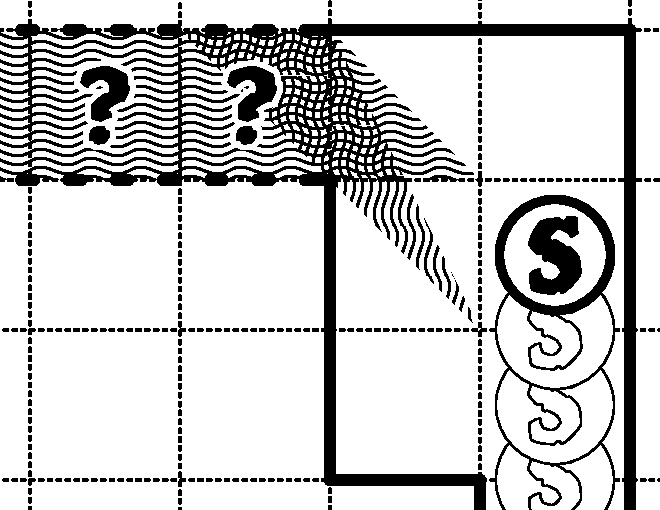
\includegraphics[width=\columnwidth]{\image{bmh/peek-expert.pdf}}
}
